\chapter{\stc{}\con{}和\scon{}绘制算法}

基于上一章的推导,可知\epsl{}可以通过检查轨迹函数$t(x)$的极值点来在图像空间中完成判定。因此,本文设计了一个算法来实现\stc{}\con{}和\scon{}绘制,并实时完成\epsl{{}的判定。在这一章中,本文将针对\con{}对整个算法流程进行总结,并对流程中每个阶段的细节进行具体的说明,再讲述如何将这套算法拓展至\scon{}上,以及如何实现进一步的线条风格化。

\begin{figure}[tbh]
    \centering
    \makebox[\textwidth][c]{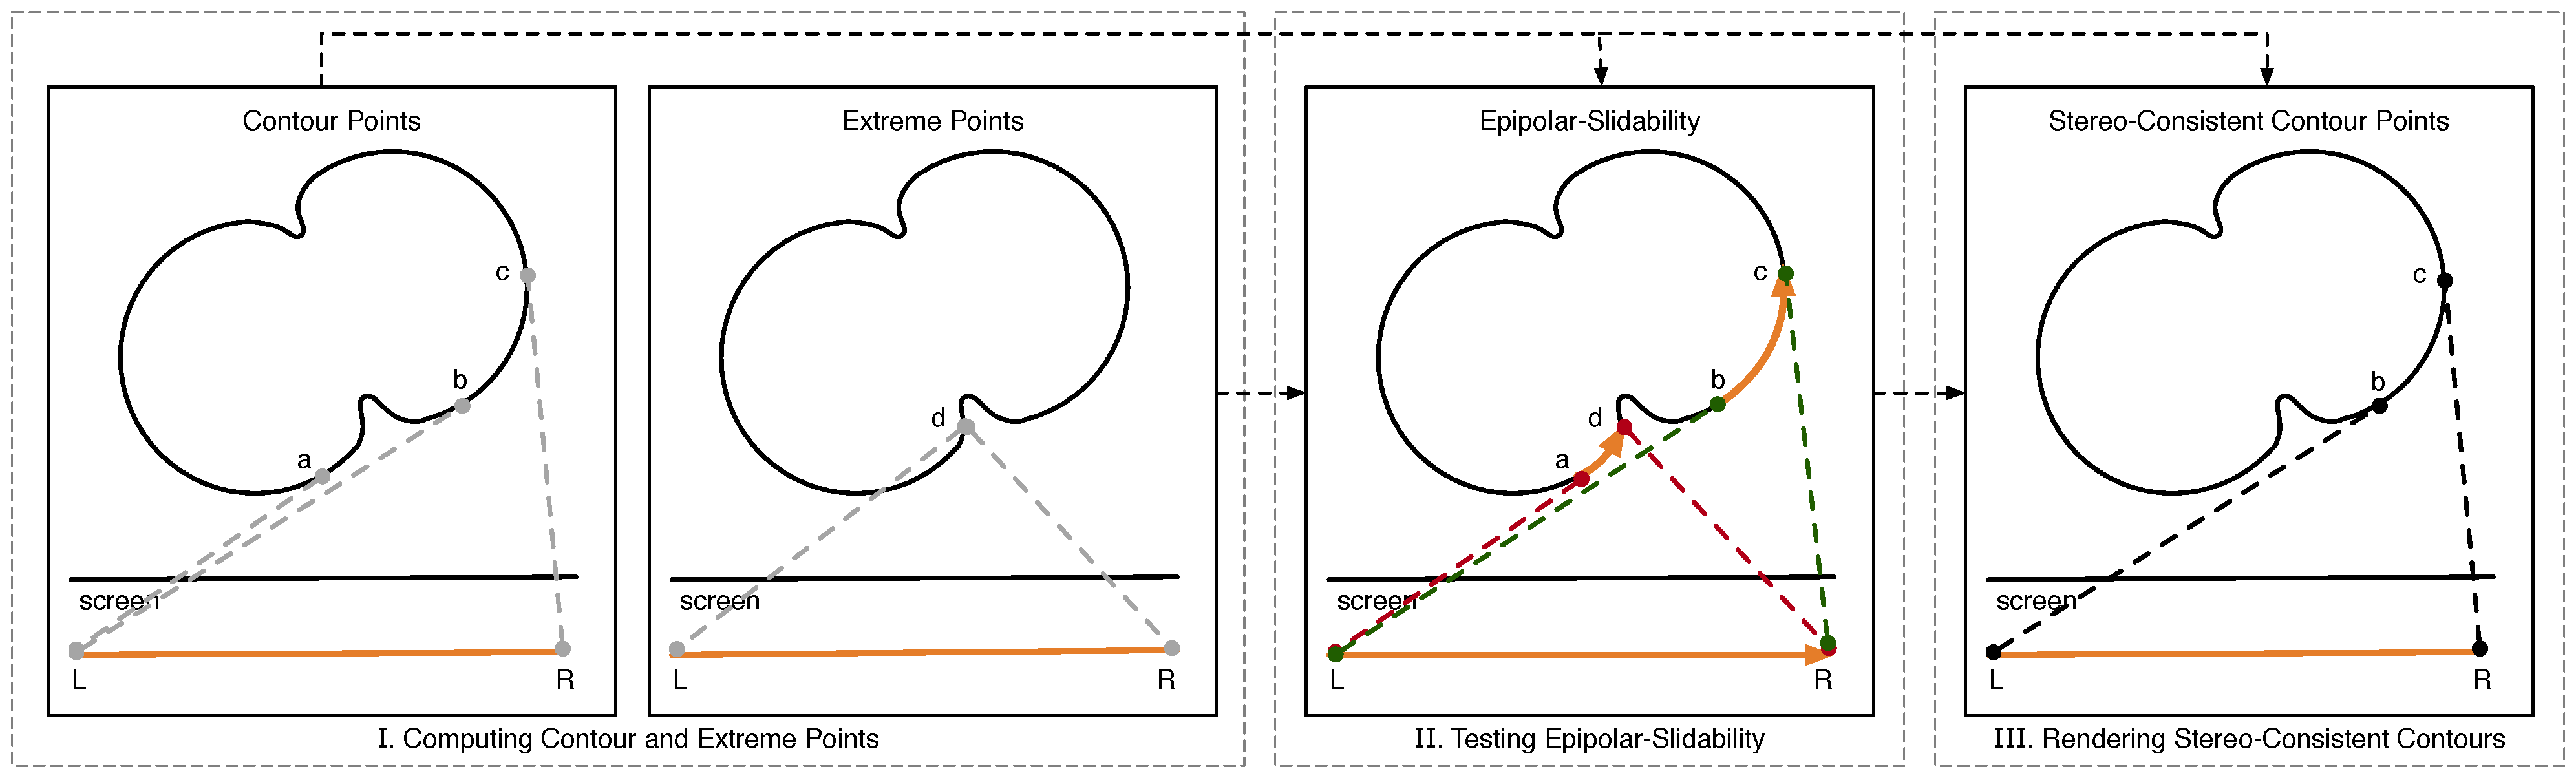
\includegraphics[width=\linewidth]{overview2}}
    \caption[算法流程说明]{\label{fig:overview2}
    算法流程说明。为了描述上的简洁,该说明只展示了从$L$到$R$计算\stc{}\con{}的过程。首先,计算出\conp{}$a$、$b$、$c$和极值点$d$。然后,本文设计的算法在图像空间中对$a$和$b$的\epsl{}进行判定,其中$a$由于遇到了$d$所以判定为不是\stc{},而$b$由于找到了对应的来自右眼的\conp{}$c$所以判定为\stc{}。最后,将\stc{}的\conp{}$b$和$c$绘制到最终展示的两眼对应图像中。
    }
\end{figure}

\autoref{fig:overview2}对本文提出的算法流程进行了说明,其中主要包含以下三个步骤:
\begin{enumerate}[label=\textbf{\Roman*.},leftmargin=*,align=left,labelwidth=\parindent,labelsep=0pt]
    \item \textbf{计算轮廓点和极值点:} 首先,在每一帧的开始阶段,遍历场景中三维模型,绘制基础的\conp{}和极值点并将它们存储到\ppll{}中。
    \item \textbf{\epsl{}的判定:} 接着,采用一个图像空间的搜索算法,通过一个全屏后处理完成对上一步得到的\con{}的\epsl{}的判定。
    \item \textbf{绘制\stc{}\con{}:} 最后,将所有的\epslb{}的\con{}绘制到两眼对应的图像中。
\end{enumerate}

\begin{figure}[tbh]
    \centering
    \makebox[\textwidth][c]{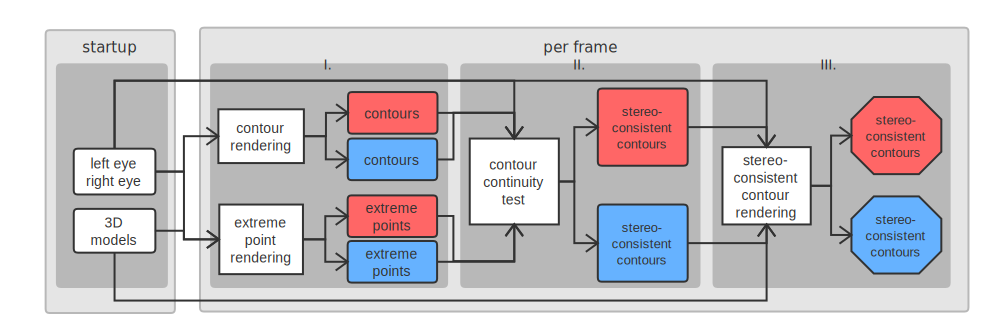
\includegraphics[width=1.2\linewidth]{overview}}
    \caption[系统总览]{\label{fig:overview}
    系统总览。蓝色/红色的正方形表示左眼/右眼的某种实例。在初始化阶段,首先载入三维模型并对对应于两眼的摄像机进行设置。在后续的每一帧中,轮廓点和极值点先是被绘制并存储到\ppll{}上,然后以这些\ppll{}作为输入进行\epsl{}的判定,最后,基于上一步得到的\epsl{}绘制出\stc{}轮廓线。}
\end{figure}

在上述算法的基础上,本文设计了一个如\autoref{fig:overview}所示实时绘制系统。下面将分别对各个阶段进行进一步的说明。

\section{计算\conp{}和极值点}

在第一个阶段,本文设计的算法先对模型进行光栅化并计算出\conp{}和极值点。如果将\scon{}也考虑在内,那么\sconp{}和对应的极值点和区间端点也需要在这个阶段完成计算。下面的两个小节将分别针对\con{}和\scon{}的计算方法进行进一步的说明。

\subsection{\con{}}

\textbf{计算轮廓点}: 在第一个阶段中计算\conp{}的方法和\autoref{sec:basic}中描述的直接绘制算法大致相同,但是不利用可见性检测对轮廓点进行剔除,而是将所有存在的\conp{}都计算出来并存储到\ppll{}中。

具体地,轮廓点的计算需要遍历场景中的三维模型进行两次绘制,其中第一次绘制用于生成可见性测试用的深度图,第二次用于轮廓点的检测与存储。其中第一次绘制生成可见性测试用的深度图的过程已经在\autoref{sec:basic}进行说明,在此不再赘述。第二次绘制的具体过程包括:在顶点着色器阶段,完成基本的投影变换的计算,并计算世界空间中的位置和法线作为顶点着色器输出信息;在几何着色器阶段,首先遍历三角形的三个顶点,计算各个顶点上的$N\cdot{V}$的值,然后按照$N\cdot{V}$的值的正负号的分布,找出其中两条边上$N\cdot{V}$的值为0的点,以这两个点作为线类型的输出图元;在片段着色器中,利用深度图完成可见性测试,然后将轮廓点处法线和视线方向的叉积、轮廓点的深度、轮廓点的可见性、所在三维模型的索引这些后续算法中需要用到的信息存储在\ppll{}中。

\textbf{计算极值点}: 极值点的计算需要根据满足$t_c'(x-)t_c'(x+) < 0$的条件去找到三维模型表面上对应的点。需要特别提出的是,本文在前一章节中的推导中得出$t_c'(x)$的表达式的正负只与$C(x)$有关。因此,本文设计的方法通过$C(x-)C(x+) < 0$而不是$t_c'(x-)t_c'(x+) < 0$来计算出\con{}对应的极值点,这样一来计算更加简单。上述的$C(x)$表示$x$处的极线上的曲率,可以在三维模型的每个三角形上以类似于通过$N\cdot{V} = 0$来找到\conp{}的方式计算出来。

然而,基于下面的原因,本文采取一种更为精确的方法来计算出这些极值点。在三维模型被光栅化之后,每个片段上的法线值是基于重心坐标对顶点法线进行插值得到的。因此,如果将一条\ec{}投影到一个三角形上,沿着投影线的法线变化必然是线性连续的,说明$C(x)$在三角形内是一个常量。因此,满足$t_c'(x-)t_c'(x+) < 0$的点不可能出现在三角形内部,而是出现在三角形与三角形之间的边上。极值点出现在三角形与三角形之间的边上的原因在于,每个三角形的法线变化的线性连续的程度是不同的,$C(x)$在跨过三角形的时候会发生突变。

因此,本文设计的极值点的计算方法如下。下面将以\autoref{fig:extreme points}为例进行说明,其中$\triangle ABC$和$\triangle ACD$是两个相邻的三角形。具体地,在顶点着色器阶段,完成基本的投影变换并将顶点在世界空间的法线和位置输出到下一个阶段;在几何着色器阶段,将边$AC$作为线类型图元进行输出,同时根据来自顶点着色器的输入,输出四个顶点$A$、$B$、$C$以及$D$上的位置和法线信息;在片段着色器阶段,假设当前处理的片段为边$AC$上的一点$x$,首先以视点为起点发射两条光线,这两条光线分别以$x$在极线方向上的两个邻点,$x+\Delta{x}$和$x-\Delta{x}$作为目标,分别计算出与$\triangle ABC$和$\triangle ACD$的两个交点。接着,在这两个交点上,可以依据各自所在三角形的三个顶点上的法线信息使用三角形重心坐标插值处该点上的法线值,并进一步计算出经过点$x$沿着极线方向的$C(x-)$和$C(x+)$的值。最后,通过$C(x-)C(x+)$的正负判定该点是否属于极值点,如果是,则将该点处的深度、所在三维模型的索引等后续算法中需要的信息存储在\ppll{}中。

需要特别指出的是,轮廓点与极值点之间可能会存在重叠,例如多个轮廓点和极值点都处在图像空间的同一个像素上。因此,本文使用了\ppll{}来分别存储同一个像素上的轮廓点和极值点。虽然\ppll{}的使用大多时候会对内存占用造成一定的影响,但是考虑到轮廓点和极值点只占图像空间中的一小部分,使用\ppll{}带来的内存占用是完全可以接受的。

\begin{figure}[tbh]
    \centering
    \subfloat[左眼]{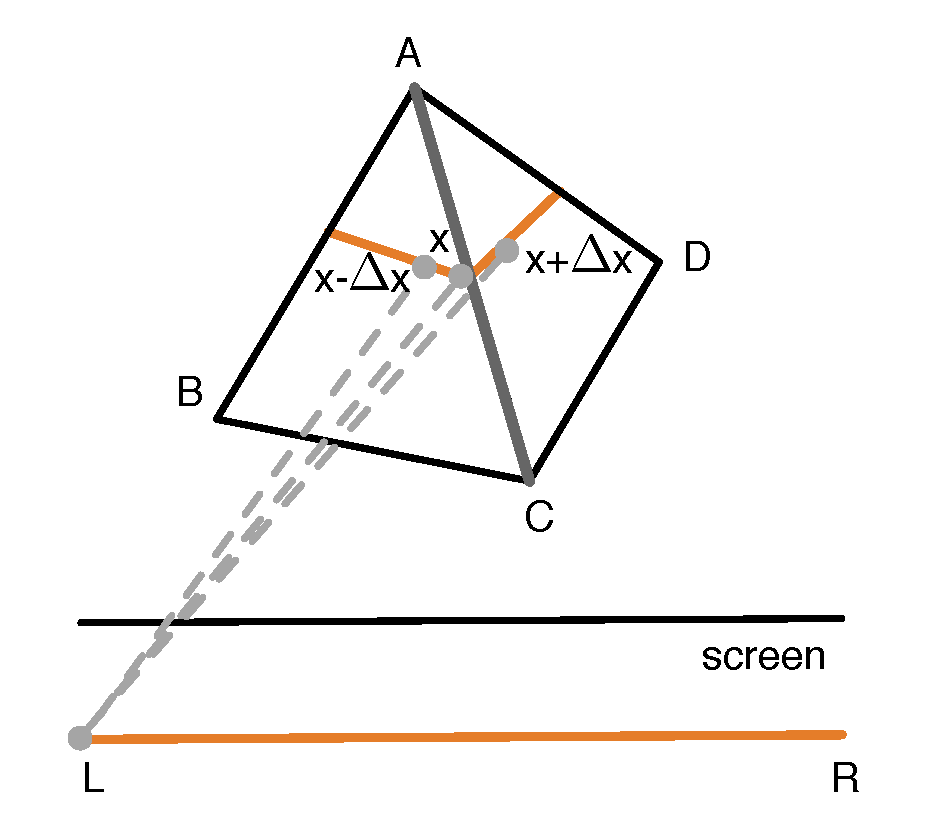
\includegraphics[width=.5\linewidth]{inflection_line_left}}
    \hfil
    \subfloat[右眼]{\includegraphics[width=.5\linewidth]{inflection_line_right}}
    \caption[轨迹函数的极值点的计算]{极值点的计算。$\triangle ABC$和$\triangle ACD$是两个相邻的三角形。本文设计的方法对位于边$AC$上的每个片段进行极值点的判定。(a) 在左眼的图像空间计算极值点。 (b) 在右眼的图像空间计算极值点。} \label{fig:extreme points}
\end{figure}

\subsection{\scon{}}

\begin{figure}[tbh]
    \centering
    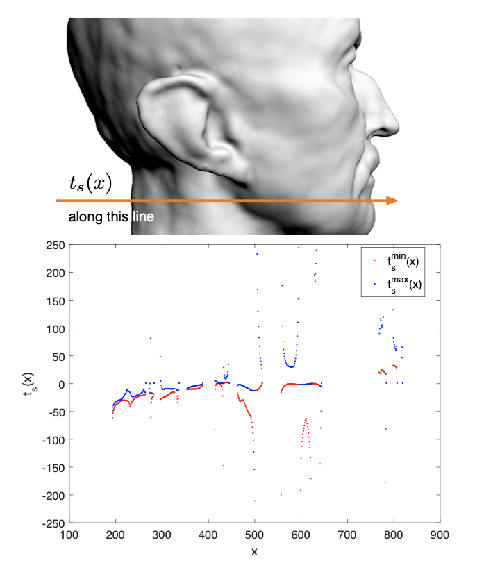
\includegraphics[width=\linewidth]{ts_example.eps}
    \caption[$t_s(x)$的一个例子]{\label{fig:continuity_example}
    $t_s(x)$的一个例子。该图表示沿着图像中某一行的$t_s(x)$的值的分布。蓝色/红色的点分别表示$t_s^{max}(x)$/$t_s^{min}(x)$的值。}
\end{figure}

\begin{figure}[tbh]
    \centering
    \includegraphics[width=.95\linewidth]{continuity}
    \caption[$t_s(x)$的连续性的三种不同情况]{在虚线所指位置上,$t_s(x)$的连续性的三种不同情况。}
    \label{fig:ts_continuity}
\end{figure}

\label{sec:suggestive_contour_algorithm}

正如本文在\ref{sec:suggestive_contour_math}中讨论的那样,对于\scon{}的\epsl{}的判定,除了需要计算轨迹函数的极值点外还需要计算出区间端点。同样地,本文采用了与绘制\con{}的方法相似的方法来计算出区间端点,也就是满足$\kappa_1\kappa_2 = 0$,或者$D_w\kappa_r = 0$,又或者$cos^{-1}(N\cdot{V}) = \theta_c$的那些点。

计算$t_s(x)$的极值点比计算$t_c(x)$的极值点要更加困难。对于\con{},基于上文\autoref{eq:curvature}所述的推导,只需要在三角形的边上进行计算即可。但是对于\scon{}而言,不存在同样的性质,所以不仅需要在边上也需要在三角形内进行计算。再者,与通过$C(x)$来找到间接地找到极值点不同,只能通过对比多个连续的$t_s(x)$的值来直接地找到$t_s(x)$的极值点。

另外,考虑到$t_s(x)$是一个对于每个点有两个取值的多值函数,必须要在通过对比$t_s(x)$的连续几个值来决定极值点前确定$t_s(x)$的多个值的连续性。为了将$t_s(x)$的两个值区分开来,本文使用$t_s^{min}(x)$和$t_s^{max}(x)$来分别表示它们中的最小值和最大值。\autoref{fig:continuity_example}展示了$t_s(x)$的一个例子。一般而言,$t_s^{min}(x)$和$t_s^{max}(x)$在大部分点上是分别连续的,但是在某些点上也会相互连续。\autoref{fig:ts_continuity}总结了$t_s(x)$的三种不同的连续情况。具体来说,本文设计的方法首先
在片段着色器中计算出三个连续的$t_s^{min}(x)$和$t_s^{max}(x)$的值,并按照这些值的关系对应到\autoref{fig:ts_continuity}中的其中一种情况。然后,对比对应的连续三个值来确定此处是否为极值点。需要特别指出的是,在\autoref{fig:ts_continuity}的情况(a)中可能会在同一个点上同时存在$t_s^{min}(x)$和$t_s^{max}(x)$的局部最小值。无论是哪一种情况,只要$t_s^{min}(x)$或者$t_s^{max}(x)$的局部极值出现,就应该将其存储为极值点。

\section{\epsl{}的判定}

\begin{figure}[tbh]
    \centering
    \subfloat[不需要重投影的搜索]{\includegraphics[width=.5\linewidth]{search_leftside_2}}
    \hfil
    \subfloat[需要重投影的搜索]{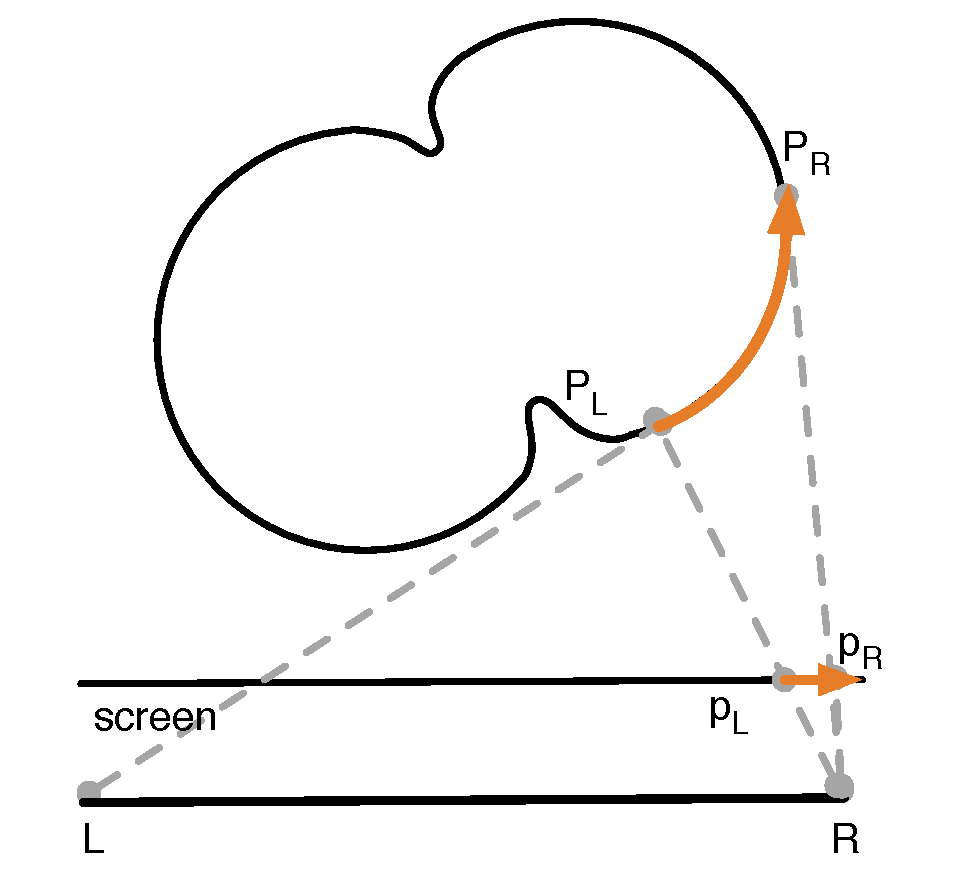
\includegraphics[width=.5\linewidth]{search_rightside}}
    \caption[遇到对应轮廓点的搜索过程]{遇到对应轮廓点的搜索过程。$p_L$和$p_R$分别表示$P_L$和$P_R$的投影。}\label{fig:succeed in image space search}
\end{figure}

\begin{figure}[tbh]
    \centering
    \subfloat[需要重投影的搜索]{\includegraphics[width=.5\linewidth]{search_leftside_fail_2}}
    \hfil
    \subfloat[需要重投影的搜索]{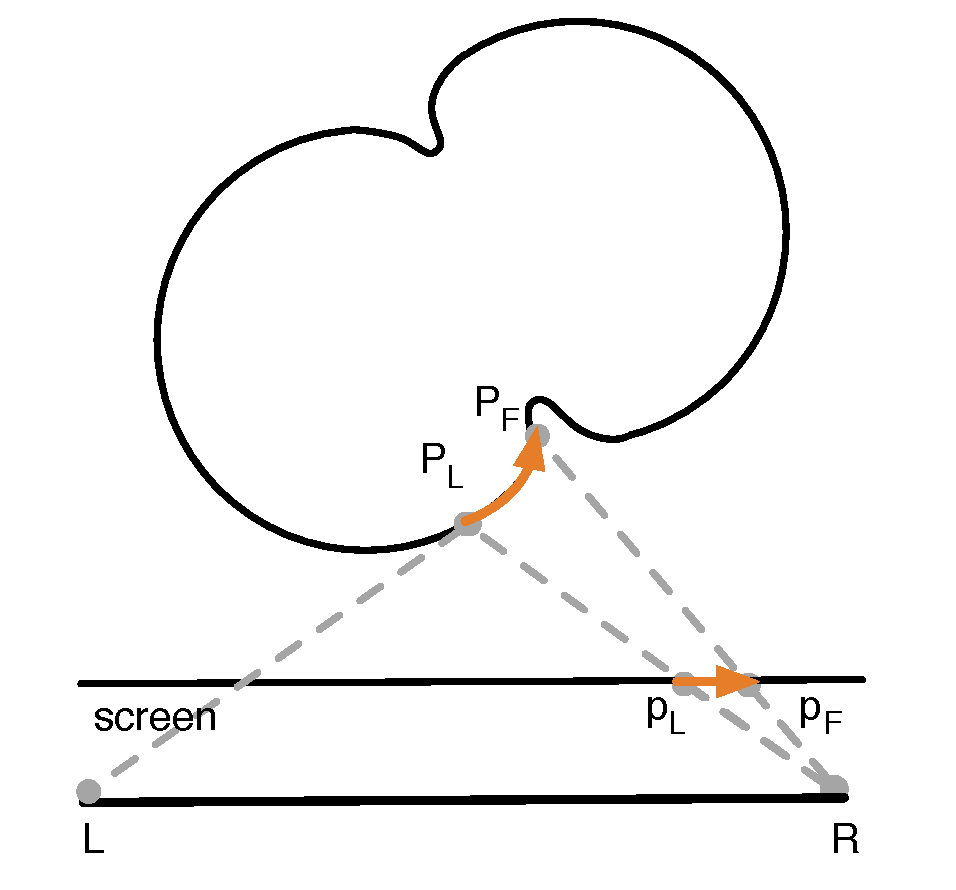
\includegraphics[width=.5\linewidth]{search_rightside_fail}}
    \caption[在极值点处停止的搜索过程]{在极值点处停止的搜索过程。$P_F$是一个极值点。$p_L$和$p_F$分别表示$P_L$和$P_F$的投影。} \label{fig:fail in image space search}
\end{figure}

\begin{figure}[tbh]
    \centering
    \includegraphics[width=0.6\linewidth]{search_occlude}
    \caption[错误匹配的排除]{\label{fig:occlude}
    由于遮挡导致的错误匹配。本文设计的方法通过物体的索引来排除这种情况。}
\end{figure}

本文使用两个全屏后处理来分别实现左眼和右眼两个图像上的\epsl{}的判定。本文设计的用于\epsl{}判定的搜索算法主要有以下三步:

\begin{enumerate}
    \item 在有需要的情况下,将\conp{}从当前视点的图像空间重投影到另一视点的图像空间。
    \item 根据\conp{}所观察的视点是左眼还是右眼,判定搜索方向(从左往右或者从右往左)。
    \item 在图像空间中逐个像素进行搜索。对于每个像素,遍历并检查存储在\ppll{}上的每个点。当遇到存有另一视点下的对应\conp{}的像素或者遇到极值点时,搜索停止。
\end{enumerate}

\autoref{fig:succeed in image space search}展示了遇到对应\conp{}的两个搜索过程,其中一个在起始位置做了重投影,另外一个没有在起始位置做重投影。而\autoref{fig:fail in image space search}展示了遇到在极值点处停止的搜索过程。下面以从$L$到$R$的搜索过程为例来阐述具体每个步骤的细节,从$R$到$L$的搜索过程是相似的。

{\textbf{重投影:} 如果\conp{}的表面法线指向视线方向的右边,则将\conp{}从当前视点的图像空间重投影到另一视点的图像空间。否则,不需要做重投影。法线指向视线方向的右边还是左边可以用明确的数学语言进行表述。如果视线方向和表面法线方向的叉积,也就是$cross(N, V)$,指向对极平面的上方,则表示\conp{}的法线方向指向视线方向的左边,反之亦然。

\textbf{搜索方向:} 搜索方向决定于将该点视为\conp{}的是左眼还是右眼。如果\conp{}是从左眼观察得到的,那么从左往右搜索。否则,从右往左搜索。

\textbf{错误匹配的排除:} 当\ec{}被其他物体所遮挡时,可能会产生错误的匹配结果。\autoref{fig:occlude}展示了这样的一个例子,其中${P^*}_R$是一个位于另外一个物体上的\conp{},${p^*}_R$是该\conp{}在图像空间上的投影。在这种情况下,搜索过程会在${p^*}_R$而不是$p_R$处结束。因此,应该被消除的\conp{}可能会因为错误的匹配而保留到最后的结果中。类似地,那些本应被消除的\conp{}可能会因为错误的匹配而被消除。为了排除这些错误的匹配,本文设计的方法将每个\conp{}和极值点所在的物体的索引也存储到\ppll{}中。有了这些索引,便可以保证在搜索过程停止在来自同一个物体的\conp{}或极值点上。

需要特别指出的是,以上说明都在以\con{}为对象进行表述。如果需要绘制\scon{},那么\scon{}的\epsl{}也是在这个阶段进行判定。对于\scon{}而言,上述的搜索过程大致相同,只是搜索过程不仅会停止在对应的轨迹函数$t_s(x)$的极值点上,还会停止在轨迹函数$t_s(x)$的区间端点上。

\section{绘制\stc{}\con{}}

在上述的\epsl{}的判定阶段结束后,便可得知所有\epslb{}的\con{}。接着,本文再将所有三维模型的\con{}以给定的线宽绘制出来,并在此过程中消去不是\epslb{}的\con{}。另外,在前者的一个关于线条可见性的工作\cite{cole2010two}中提到的样条测试方法的基础上,本文采用了与之相似的策略来减少结果的瑕疵,即通过使用多个沿着\con{}方向的\epsl{}的探针来减少锯齿和线条的断裂。如果有多个\conp{}处在同一个像素上的\ppll{}上,那么选择深度最低的那个作为样本。在这一阶段中,所有对于\con{}的操作都可以同样地采用到\scon{}上,所以可以将\stc{}\scon{}同时一次过绘制出来。

\section{线条的风格化绘制}

Kim等人在他们的工作\cite{kim2013stereoscopic}中通过将风格化参数从一个视点的图像空间传递到另一个视点的图像空间的方法来实现风格化的轮廓线。Bukenberger等人则在他们的物体空间的方法\cite{bukenberger2018stereo}中采取了根据物体空间属性来确定风格化参数的方法。本文提出的方法也同样支持\con{}和\scon{}的风格化绘制。本文采用了一种启发式的组合方法来解决这个问题,即在图像空间中传递纹理坐标,并在物体空间中确定除纹理坐标以外的其他风格化参数。具体而言,纹理坐标的传递通过上述第二阶段的轮廓点匹配来完成,而其他的风格化参数则在第三个阶段中基于物体空间的几何特征来确定。对于\scon{}而言,以上表述也同样成立。